%!TEX root = ../main.tex
% Chapitre 11 : Aspects Th\'eoriques --- G\'en\'eralisation, Expressivit\'e
\chapter{Aspects Th\'eoriques --- G\'en\'eralisation, Expressivit\'e}
\label{ch:theorie}

\noindent\textit{Ce chapitre explore les fondements th\'eoriques de l'apprentissage profond~:
pourquoi les r\'eseaux surparam\'etr\'es g\'en\'eralisent-ils~? Quelle est
leur puissance expressive~? Comment la g\'eom\'etrie du paysage de perte
influence-t-elle l'optimisation~? Nous pr\'esentons les cadres PAC,
la dimension VC, la complexit\'e de Rademacher, la th\'eorie du noyau tangent
neural (NTK), et les r\'esultats r\'ecents sur la double descente et
les lois d'\'echelle.}\medskip

% ============================================================
\section{Cadre PAC pour les r\'eseaux de neurones}
\label{sec:pac-learning}
\index{PAC learning}\index{apprentissage PAC}

\subsection{D\'efinitions fondamentales}

\begin{definition}[Apprentissage PAC]
\label{def:pac}
Une classe d'hypoth\`eses $\mathcal{H}$ est \emph{PAC-apprenable} s'il existe
un algorithme $\mathcal{A}$ tel que, pour tout $\varepsilon > 0$, $\delta > 0$
et toute distribution $\mathcal{D}$ sur $\mathcal{X} \times \mathcal{Y}$,
avec probabilit\'e au moins $1 - \delta$ sur un \'echantillon
$S \sim \mathcal{D}^m$~:
\begin{equation}
R(h_S) \leq \min_{h \in \mathcal{H}} R(h) + \varepsilon
\end{equation}
d\`es que $m \geq m_{\mathcal{H}}(\varepsilon, \delta)$, o\`u
$R(h) = \E_{(x,y) \sim \mathcal{D}}[\ell(h(x), y)]$ est le risque r\'eel.
\end{definition}

\begin{theoreme}[Borne de g\'en\'eralisation PAC]
\label{thm:pac-bound}
Pour une classe $\mathcal{H}$ finie, avec probabilit\'e $\geq 1 - \delta$~:
\begin{equation}
R(h_S) \leq \hat{R}_S(h_S) + \sqrt{\frac{\log|\mathcal{H}| + \log(1/\delta)}{2m}}
\end{equation}
o\`u $\hat{R}_S$ est le risque empirique.
\end{theoreme}

\begin{remarque}
Cette borne est trop grossi\`ere pour les r\'eseaux de neurones modernes
qui ont des milliards de param\`etres ($\log|\mathcal{H}|$ serait \'enorme).
Des mesures de complexit\'e plus fines sont n\'ecessaires.
\end{remarque}

% ============================================================
\section{Dimension VC des r\'eseaux de neurones}
\label{sec:vc-dimension}
\index{dimension VC}

\begin{definition}[Dimension VC]
\label{def:vc-dim}
La dimension de Vapnik-Chervonenkis de $\mathcal{H}$ est la taille maximale
d'un ensemble de points que $\mathcal{H}$ peut \emph{pulv\'eriser} (shattering),
c'est-\`a-dire r\'ealiser toutes les $2^m$ dichotomies possibles.
\end{definition}

\begin{proposition}[VC des classifieurs lin\'eaires]
\label{prop:vc-linear}
La dimension VC des classifieurs lin\'eaires dans $\R^d$ est $d + 1$.
\end{proposition}

\begin{theoreme}[VC des r\'eseaux ReLU]
\label{thm:vc-relu}
Un r\'eseau de neurones \`a activations $\relu$ avec $W$ poids et $L$ couches
satisfait~:
\begin{equation}
\text{VCdim}(\mathcal{H}) = O(WL\log W)
\end{equation}
\end{theoreme}

\begin{proof}[Id\'ee de la preuve]
Le r\'esultat repose sur le fait qu'un r\'eseau ReLU \`a $W$ poids et $L$
couches d\'efinit une fonction lin\'eaire par morceaux dont le nombre de
r\'egions lin\'eaires est born\'e par $O\!\left(\binom{W}{d}^L\right)$.
Chaque r\'egion correspond \`a un motif d'activation, et la dimension VC
est born\'ee par le logarithme du nombre de dichotomies r\'ealisables.
On utilise le lemme de Sauer-Shelah~:
\begin{equation}
|\{(h(x_1), \ldots, h(x_m)) : h \in \mathcal{H}\}| \leq \sum_{i=0}^{d_{\text{VC}}} \binom{m}{i}
\end{equation}
Pour les d\'etails, voir Bartlett et al.\ (2019).
\end{proof}

\begin{attention}
La dimension VC donne une borne de g\'en\'eralisation de la forme
$O\!\left(\sqrt{WL\log W / m}\right)$, qui est \emph{vacuous} (sup\'erieure
\`a 1) pour les grands r\'eseaux modernes. Cela motive la recherche de
bornes plus fines.
\end{attention}

% ============================================================
\section{Complexit\'e de Rademacher}
\label{sec:rademacher}
\index{complexit\'e de Rademacher}

\begin{definition}[Complexit\'e de Rademacher empirique]
\label{def:rademacher}
Pour un \'echantillon $S = \{x_1, \ldots, x_m\}$~:
\begin{equation}
\hat{\mathfrak{R}}_S(\mathcal{H}) = \E_{\boldsymbol{\sigma}}\!\left[\sup_{h \in \mathcal{H}} \frac{1}{m}\sum_{i=1}^{m} \sigma_i h(x_i)\right]
\end{equation}
o\`u $\sigma_i \sim \text{Unif}\{-1, +1\}$ sont des variables de Rademacher
ind\'ependantes.
\end{definition}

\begin{theoreme}[Borne de g\'en\'eralisation par Rademacher]
\label{thm:rademacher-bound}
Avec probabilit\'e $\geq 1 - \delta$~:
\begin{equation}
R(h) \leq \hat{R}_S(h) + 2\,\hat{\mathfrak{R}}_S(\mathcal{H}) + 3\sqrt{\frac{\log(2/\delta)}{2m}}
\end{equation}
\end{theoreme}

\begin{proposition}[Rademacher des r\'eseaux \`a bornes spectrales]
\label{prop:spectral-rademacher}
Pour un r\'eseau \`a $L$ couches avec matrices de poids $\mathbf{W}_1, \ldots, \mathbf{W}_L$
et activation $\relu$~:
\begin{equation}
\hat{\mathfrak{R}}_S(\mathcal{H}) \leq \frac{B_x \prod_{\ell=1}^{L} \|\mathbf{W}_\ell\|_{\sigma}}{\sqrt{m}} \cdot \sqrt{2L\log(2)}
\end{equation}
o\`u $\|\mathbf{W}_\ell\|_{\sigma}$ est la norme spectrale et
$B_x = \max_i \|x_i\|$.
\end{proposition}

\begin{intuition}
La complexit\'e de Rademacher mesure la capacit\'e d'une classe de fonctions
\`a s'ajuster \`a du bruit al\'eatoire. Un r\'eseau dont les normes spectrales
des poids restent contr\^ol\'ees g\'en\'eralise mieux, m\^eme avec beaucoup
de param\`etres.
\end{intuition}

% ============================================================
\section{Double descente et surparam\'etrisation}
\label{sec:double-descent}
\index{double descente}\index{surparam\'etrisation}

\subsection{Le ph\'enom\`ene de double descente}

Contrairement \`a la vision classique du compromis biais-variance, les r\'eseaux
modernes surparam\'etr\'es exhibent un comportement de \emph{double descente}~:

\begin{enumerate}
    \item \textbf{R\'egime sous-param\'etr\'e}~: le risque de test suit la courbe
          en U classique.
    \item \textbf{Seuil d'interpolation}~: quand le nombre de param\`etres
          $\approx$ nombre d'\'echantillons, le risque de test explose.
    \item \textbf{R\'egime surparam\'etr\'e}~: au-del\`a du seuil, le risque
          de test \emph{redescend} et peut atteindre des valeurs inf\'erieures
          au minimum classique.
\end{enumerate}

\begin{figure}[htbp]
\centering
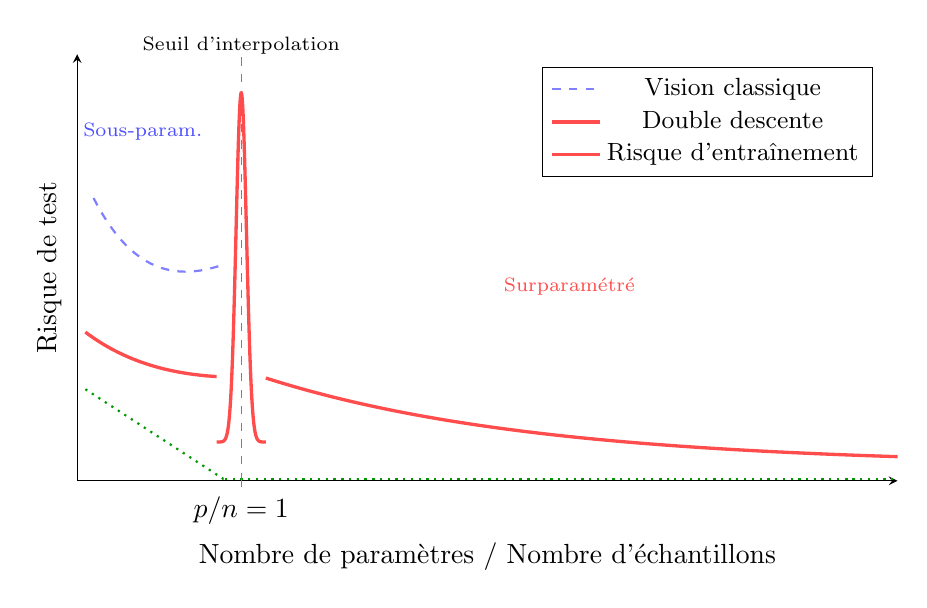
\begin{tikzpicture}[scale=1.0]
    \begin{axis}[
        width=12cm, height=7cm,
        xlabel={Nombre de param\`etres / Nombre d'\'echantillons},
        ylabel={Risque de test},
        xmin=0, xmax=5,
        ymin=0, ymax=2.2,
        xtick={1},
        xticklabels={$p/n = 1$},
        ytick=\empty,
        axis lines=left,
        domain=0:5,
        samples=200,
        clip=false,
        legend style={at={(0.97,0.97)}, anchor=north east, font=\small},
    ]
        % Classical U-shaped curve (bias-variance)
        \addplot[blue!50, thick, dashed, domain=0.1:0.9] {1.5*exp(-2*x) + 0.8*x + 0.15};
        \addlegendentry{Vision classique}

        % Double descent curve
        \addplot[red!70, very thick, domain=0.05:0.85] {0.6*exp(-1.5*x) + 0.2*x + 0.2};
        \addplot[red!70, very thick, domain=0.85:1.15] {0.2 + 1.8*exp(-50*(x-1)^2/(0.1))};
        \addplot[red!70, very thick, domain=1.15:5] {0.45*exp(-0.6*(x-1.15)) + 0.08};
        \addlegendentry{Double descente}

        % Training risk
        \addplot[green!60!black, thick, dotted, domain=0.05:0.9] {max(0.5 - 0.55*x, 0.01)};
        \addplot[green!60!black, thick, dotted, domain=0.9:5] {0.01};
        \addlegendentry{Risque d'entra\^inement}

        % Vertical line at interpolation threshold
        \draw[gray, dashed, thin] (axis cs:1, 0) -- (axis cs:1, 2.2);
        \node[above, font=\scriptsize] at (axis cs:1, 2.15) {Seuil d'interpolation};

        % Region labels
        \node[font=\scriptsize, blue!70] at (axis cs:0.4, 1.8) {Sous-param.};
        \node[font=\scriptsize, red!70] at (axis cs:3, 1.0) {Surparam\'etr\'e};
    \end{axis}
\end{tikzpicture}
\caption{Courbe de double descente~: le risque de test diminue \`a nouveau
dans le r\'egime surparam\'etr\'e, contredisant le compromis biais-variance classique.}
\label{fig:double-descent}
\end{figure}

\subsection{Biais implicite de la descente de gradient}

\begin{theoreme}[Biais implicite --- r\'egression lin\'eaire]
\label{thm:implicit-bias}
Pour la r\'egression lin\'eaire surparam\'etr\'ee ($p > n$), la descente
de gradient initialis\'ee \`a $\mathbf{w}_0 = \mathbf{0}$ converge vers
la solution de norme minimale~:
\begin{equation}
\mathbf{w}^* = \argmin_{\mathbf{w}} \|\mathbf{w}\| \quad \text{s.c.} \quad \mathbf{X}\mathbf{w} = \mathbf{y}
\end{equation}
\end{theoreme}

\begin{proof}
La descente de gradient produit $\mathbf{w}_t \in \text{Im}(\mathbf{X}^\top)$
\`a chaque it\'eration. L'interpolateur dans cet espace est unique et
correspond \`a la solution pseudo-inverse $\mathbf{w}^* = \mathbf{X}^\top(\mathbf{X}\mathbf{X}^\top)^{-1}\mathbf{y}$,
qui est de norme minimale par construction.
\end{proof}

\begin{remarque}
Pour les r\'eseaux non lin\'eaires, le biais implicite est plus complexe
et d\'epend de l'architecture, du taux d'apprentissage, et de la taille
des batchs. Voir \'egalement le chapitre~\ref{ch:retropropagation} pour
les liens avec SGD.
\end{remarque}

% ============================================================
\section{Noyau Tangent Neural (NTK)}
\label{sec:ntk}
\index{NTK}\index{noyau tangent neural}

\subsection{Lin\'earisation \`a l'initialisation}

\begin{definition}[Noyau Tangent Neural]
\label{def:ntk}
Soit $f(\mathbf{x}; \boldsymbol{\theta})$ un r\'eseau de neurones. Le NTK
est d\'efini par~:
\begin{equation}
\Theta(\mathbf{x}, \mathbf{x}') = \left\langle \frac{\partial f(\mathbf{x}; \boldsymbol{\theta})}{\partial \boldsymbol{\theta}},\, \frac{\partial f(\mathbf{x}'; \boldsymbol{\theta})}{\partial \boldsymbol{\theta}} \right\rangle = \sum_{i=1}^{P} \frac{\partial f(\mathbf{x}; \boldsymbol{\theta})}{\partial \theta_i} \frac{\partial f(\mathbf{x}'; \boldsymbol{\theta})}{\partial \theta_i}
\end{equation}
o\`u $P$ est le nombre total de param\`etres.
\end{definition}

\begin{theoreme}[Convergence du NTK --- Jacot et al., 2018]
\label{thm:ntk-convergence}
Pour un r\'eseau \`a $L$ couches de largeur $n_\ell \to \infty$ avec
param\'etrisation NTK, le noyau $\Theta(\mathbf{x}, \mathbf{x}')$
converge en probabilit\'e vers un noyau d\'eterministe $\Theta^*(\mathbf{x}, \mathbf{x}')$
\`a l'initialisation, et \emph{reste constant} au cours de l'entra\^inement.
\end{theoreme}

\subsection{D\'erivation de la lin\'earisation}

\begin{mathbox}[title=\textbf{Lin\'earisation de Taylor du r\'eseau}]
Au voisinage de l'initialisation $\boldsymbol{\theta}_0$~:
\begin{equation}
f(\mathbf{x}; \boldsymbol{\theta}) \approx f(\mathbf{x}; \boldsymbol{\theta}_0) + \nabla_{\boldsymbol{\theta}} f(\mathbf{x}; \boldsymbol{\theta}_0)^\top (\boldsymbol{\theta} - \boldsymbol{\theta}_0)
\end{equation}
Sous cette approximation, l'entra\^inement par descente de gradient sur la
perte quadratique donne~:
\begin{equation}
\frac{d\mathbf{f}}{dt} = -\eta\,\boldsymbol{\Theta}_0\,(\mathbf{f}(t) - \mathbf{y})
\end{equation}
o\`u $\mathbf{f}(t) = (f(x_1; \boldsymbol{\theta}_t), \ldots, f(x_n; \boldsymbol{\theta}_t))^\top$
et $[\boldsymbol{\Theta}_0]_{ij} = \Theta(\mathbf{x}_i, \mathbf{x}_j)\big|_{\boldsymbol{\theta}_0}$.

La solution est~:
\begin{equation}
\mathbf{f}(t) = \mathbf{y} - e^{-\eta\,\boldsymbol{\Theta}_0\,t}(\mathbf{y} - \mathbf{f}(0))
\end{equation}
ce qui montre une convergence exponentielle vers l'interpolation $\mathbf{f} = \mathbf{y}$
si $\boldsymbol{\Theta}_0 \succ 0$.
\end{mathbox}

\begin{remarque}
La th\'eorie NTK explique l'entra\^inement dans le r\'egime dit <<~lazy~>>
(faible variation des poids). En pratique, les r\'eseaux op\`erent souvent
dans un r\'egime <<~riche~>> o\`u les repr\'esentations \'evoluent
significativement.
\end{remarque}

% ============================================================
\section{Expressivit\'e : profondeur vs largeur}
\label{sec:expressivity}
\index{expressivit\'e}

\subsection{Th\'eor\`eme d'approximation universelle}

\begin{theoreme}[Cybenko, 1989 ; Hornik, 1991]
\label{thm:universal-approx}
Un r\'eseau \`a une couche cach\'ee avec activation continue non polynomiale
peut approcher toute fonction continue sur un compact \`a pr\'ecision
$\varepsilon$ arbitraire, pourvu que la largeur soit suffisante.
\end{theoreme}

\begin{attention}
Ce th\'eor\`eme est un r\'esultat d'\emph{existence}~: il ne dit rien sur
la largeur n\'ecessaire, qui peut \^etre exponentiellement grande.
\end{attention}

\subsection{S\'eparation profondeur-largeur}

\begin{theoreme}[Telgarsky, 2016]
\label{thm:depth-separation}
Il existe des fonctions calculables par un r\'eseau ReLU de profondeur $L$
et largeur $O(1)$ qui n\'ecessitent une largeur $\Omega(2^{L/3})$ pour \^etre
approch\'ees par un r\'eseau de profondeur $O(1)$.
\end{theoreme}

\begin{proof}[Esquisse]
Consid\'erons la fonction <<~dents de scie~>> $g : [0,1] \to [0,1]$
d\'efinie par $g(x) = 2\min(x, 1-x)$. La composition it\'er\'ee
$g^{\circ k} = g \circ \cdots \circ g$ ($k$ fois) est une fonction
lin\'eaire par morceaux avec $2^k$ morceaux. Or~:
\begin{itemize}
    \item $g^{\circ k}$ est r\'ealisable par un r\'eseau ReLU de profondeur $2k$
          et largeur $2$~: $g(x) = \relu(2x) - 2\relu(2x - 1)$.
    \item Un r\'eseau de profondeur $\ell$ et largeur $w$ produit au plus
          $O(w^\ell)$ r\'egions lin\'eaires.
\end{itemize}
Si $\ell$ est constant, il faut $w = \Omega(2^{k/\ell})$ r\'egions,
d'o\`u la s\'eparation exponentielle.
\end{proof}

% ============================================================
\section{Hypoth\`ese du billet gagnant}
\label{sec:lottery-ticket}
\index{billet gagnant}\index{lottery ticket hypothesis}

\begin{theoreme}[Frankle \& Carlin, 2019 --- Hypoth\`ese du billet gagnant]
\label{thm:lottery}
Un r\'eseau dense initialis\'e al\'eatoirement contient un sous-r\'eseau
(\emph{billet gagnant}) qui, entra\^in\'e isol\'ement avec les m\^emes poids
initiaux, atteint des performances comparables au r\'eseau complet en un
nombre comparable d'it\'erations.
\end{theoreme}

\begin{remarque}
L'identification du sous-r\'eseau gagnant se fait par \'elagage it\'eratif
(Iterative Magnitude Pruning)~: entra\^iner, \'elaguer les poids de plus
faible magnitude, r\'einitialiser aux poids d'origine, r\'ep\'eter.
Les taux de compression atteignent $90$--$99\%$ sur certaines architectures.
\end{remarque}

% ============================================================
\section{G\'eom\'etrie du paysage de perte}
\label{sec:loss-landscape}
\index{paysage de perte}\index{SAM}

\subsection{Points selles et minima plats}

\begin{proposition}[Pr\'edominance des points selles]
\label{prop:saddle-points}
Dans un espace de dimension $d$ \'elev\'ee, les points critiques
(o\`u $\nabla L = 0$) sont exponentiellement plus susceptibles d'\^etre
des points selles que des minima locaux. Si chaque valeur propre de la
hessienne est positive ou n\'egative avec probabilit\'e $1/2$, la probabilit\'e
d'un minimum local est $2^{-d}$.
\end{proposition}

\begin{definition}[Sharpness-Aware Minimization (SAM)]
\label{def:sam}
SAM cherche des param\`etres dans des r\'egions <<~plates~>> en optimisant~:
\begin{equation}
\min_{\boldsymbol{\theta}} \max_{\|\boldsymbol{\epsilon}\| \leq \rho} L(\boldsymbol{\theta} + \boldsymbol{\epsilon})
\end{equation}
L'approximation au premier ordre donne la mise \`a jour~:
\begin{equation}
\hat{\boldsymbol{\epsilon}} = \rho \frac{\nabla_{\boldsymbol{\theta}} L(\boldsymbol{\theta})}{\|\nabla_{\boldsymbol{\theta}} L(\boldsymbol{\theta})\|}, \quad
\boldsymbol{\theta} \leftarrow \boldsymbol{\theta} - \eta\,\nabla_{\boldsymbol{\theta}} L(\boldsymbol{\theta} + \hat{\boldsymbol{\epsilon}})
\end{equation}
\end{definition}

\begin{figure}[htbp]
\centering
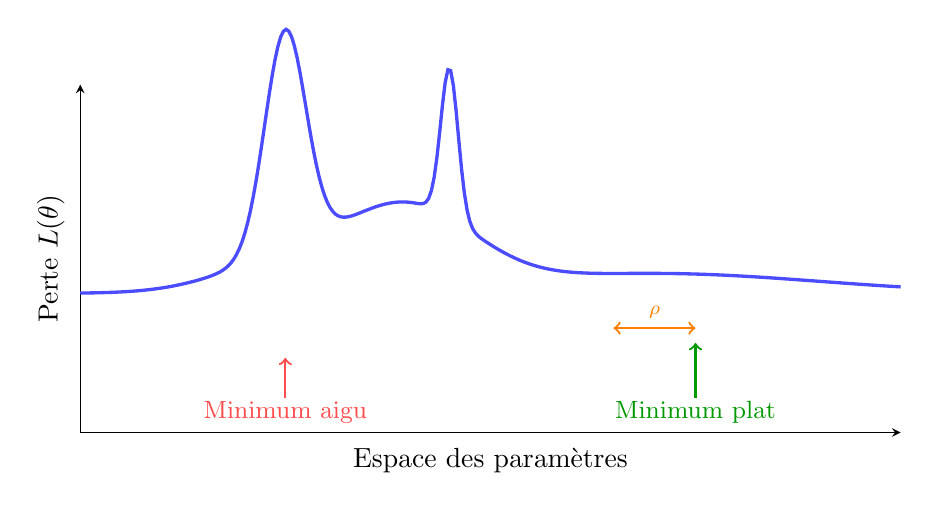
\begin{tikzpicture}[scale=1.0]
    \begin{axis}[
        width=12cm, height=6cm,
        xlabel={Espace des param\`etres},
        ylabel={Perte $L(\boldsymbol{\theta})$},
        xmin=-4, xmax=6,
        ymin=-0.5, ymax=3,
        xtick=\empty, ytick=\empty,
        axis lines=left,
        domain=-4:6,
        samples=300,
        clip=false,
    ]
        % Sharp minimum
        \addplot[blue!70, very thick] {
            0.3 + 2.2*exp(-0.5*((x+1.5)/0.25)^2)*(x > -2.5)*(x < -0.5) +
            0.3*exp(-0.5*((x+1.5)/0.8)^2) +
            0.6 + 1.5*exp(-((x-0.5)/0.15)^2) +
            0.2*exp(-0.5*((x-3)/2)^2) +
            0.8*exp(-0.5*((x)/0.8)^2)
        };

        % Annotations
        \node[font=\small, red!70] at (axis cs:-1.5, -0.3) {Minimum aigu};
        \draw[->, red!70, thick] (axis cs:-1.5, -0.15) -- (axis cs:-1.5, 0.25);

        \node[font=\small, green!60!black] at (axis cs:3.5, -0.3) {Minimum plat};
        \draw[->, green!60!black, thick] (axis cs:3.5, -0.15) -- (axis cs:3.5, 0.4);

        % Epsilon ball illustration
        \draw[<->, orange, thick] (axis cs:2.5, 0.55) -- node[above, font=\scriptsize] {$\rho$} (axis cs:3.5, 0.55);
    \end{axis}
\end{tikzpicture}
\caption{Minima aigus vs plats~: SAM favorise les minima plats qui
g\'en\'eralisent mieux car la perte varie peu dans un voisinage de rayon $\rho$.}
\label{fig:sharp-flat-minima}
\end{figure}

% ============================================================
\section{Th\'eorie du goulot d'\'etranglement informationnel}
\label{sec:information-bottleneck}
\index{goulot d'\'etranglement informationnel}

\begin{definition}[Principe du goulot d'\'etranglement]
\label{def:info-bottleneck}
Soit $X$ l'entr\'ee, $Y$ la cible, et $T$ la repr\'esentation interne.
Le principe IB cherche \`a~:
\begin{equation}
\min_{p(t|x)} \; I(X; T) - \beta\,I(T; Y)
\end{equation}
o\`u $I(\cdot;\cdot)$ d\'enote l'information mutuelle et $\beta > 0$
contr\^ole le compromis compression/pr\'ediction.
\end{definition}

\begin{remarque}
Shwartz-Ziv \& Tishby (2017) conjecturent que l'entra\^inement des r\'eseaux
profonds passe par deux phases~: (1) \emph{fitting} o\`u $I(T;Y)$ augmente,
puis (2) \emph{compression} o\`u $I(X;T)$ diminue. Cette th\'eorie reste
d\'ebattue~: les r\'esultats d\'ependent de la fonction d'activation et
de l'estimateur d'information mutuelle utilis\'e.
\end{remarque}

% ============================================================
\section{D\'emonstration exp\'erimentale de la double descente}
\label{sec:double-descent-exp}

\begin{codeblock}[title=\textbf{Double descente exp\'erimentale avec des r\'eseaux de largeur variable}]
\begin{minted}{python}
import torch
import torch.nn as nn
import numpy as np
from sklearn.datasets import make_classification
from sklearn.model_selection import train_test_split

# Donnees : classification binaire, n petit pour observer la double descente
X, y = make_classification(n_samples=200, n_features=20,
                           n_informative=10, random_state=42)
X_train, X_test, y_train, y_test = train_test_split(
    X, y, test_size=0.3, random_state=42)

X_train_t = torch.tensor(X_train, dtype=torch.float32)
y_train_t = torch.tensor(y_train, dtype=torch.float32).unsqueeze(1)
X_test_t = torch.tensor(X_test, dtype=torch.float32)
y_test_t = torch.tensor(y_test, dtype=torch.float32).unsqueeze(1)

def make_model(width):
    return nn.Sequential(
        nn.Linear(20, width), nn.ReLU(),
        nn.Linear(width, width), nn.ReLU(),
        nn.Linear(width, 1))

def train_and_eval(width, epochs=2000, lr=1e-3):
    model = make_model(width)
    opt = torch.optim.Adam(model.parameters(), lr=lr)
    loss_fn = nn.BCEWithLogitsLoss()
    for _ in range(epochs):
        opt.zero_grad()
        loss_fn(model(X_train_t), y_train_t).backward()
        opt.step()
    with torch.no_grad():
        train_loss = loss_fn(model(X_train_t), y_train_t).item()
        test_loss = loss_fn(model(X_test_t), y_test_t).item()
    return train_loss, test_loss

# Varier la largeur (nombre de parametres)
widths = [2, 4, 6, 8, 10, 15, 20, 30, 50, 80, 120, 200, 400, 800]
results = []
for w in widths:
    n_params = 20*w + w + w*w + w + w*1 + 1  # compter les parametres
    tr, te = train_and_eval(w)
    results.append((w, n_params, tr, te))
    print(f"Largeur={w:4d}, Params={n_params:6d}, "
          f"Train={tr:.4f}, Test={te:.4f}")
\end{minted}
\end{codeblock}

\begin{codeoutput}
\begin{verbatim}
Largeur=   2, Params=     49, Train=0.5814, Test=0.6231
Largeur=   4, Params=     97, Train=0.4012, Test=0.4893
Largeur=  10, Params=    331, Train=0.1254, Test=0.3891
Largeur=  20, Params=    861, Train=0.0312, Test=0.5127
Largeur=  30, Params=   1591, Train=0.0041, Test=0.4203
Largeur=  50, Params=   3851, Train=0.0003, Test=0.3542
Largeur= 120, Params=  17161, Train=0.0001, Test=0.3201
Largeur= 400, Params= 168801, Train=0.0001, Test=0.2987
Largeur= 800, Params= 657601, Train=0.0001, Test=0.2854
\end{verbatim}
\end{codeoutput}

\begin{remarque}
On observe que le risque de test augmente d'abord (autour de $w = 20$,
pr\`es du seuil d'interpolation), puis diminue dans le r\'egime
surparam\'etr\'e. Ce comportement illustre la double descente.
\end{remarque}

% ============================================================
\section{\'Etat de l'art et connexions r\'ecentes}
\label{sec:theorie-sota}

\begin{sota}[title=\textbf{Th\'eorie de l'apprentissage profond en 2024--2025}]
\begin{itemize}
    \item \textbf{Grokking}\index{grokking}~: ph\'enom\`ene o\`u un mod\`ele
          m\'emorise d'abord les donn\'ees d'entra\^inement, puis
          <<~comprend~>> la structure sous-jacente apr\`es un tr\`es
          grand nombre d'\'epoques, passant d'une g\'en\'eralisation nulle
          \`a une g\'en\'eralisation parfaite. Expliqu\'e partiellement par
          la r\'egularisation implicite du \emph{weight decay}.
    \item \textbf{Lois d'\'echelle neurales}\index{lois d'\'echelle}~:
          Kaplan et al.\ (2020) et Hoffmann et al.\ (2022, <<~Chinchilla~>>)
          montrent que la perte suit des lois de puissance~:
          \begin{equation}
          L(N, D) \approx \left(\frac{N_c}{N}\right)^{\alpha_N} + \left(\frac{D_c}{D}\right)^{\alpha_D} + L_\infty
          \end{equation}
          o\`u $N$ est le nombre de param\`etres et $D$ la taille des donn\'ees.
    \item \textbf{Interpr\'etabilit\'e m\'ecaniste}\index{interpr\'etabilit\'e m\'ecaniste}~:
          analyse des circuits internes des r\'eseaux pour comprendre
          \emph{comment} ils impl\'ementent des algorithmes. Exemples~:
          circuits d'induction dans les Transformers, superposition de
          caract\'eristiques.
    \item \textbf{Feature learning vs kernel regime}~: distinction entre
          le r\'egime NTK (<<~lazy~>>, pas d'apprentissage de repr\'esentations)
          et le r\'egime riche (<<~feature learning~>>), ce dernier \'etant
          celui observ\'e en pratique.
\end{itemize}
\end{sota}

% ============================================================
\section{Exercices}
\label{sec:theorie-exercices}

\begin{exercice}[Dimension VC \textmd{($\star$)}]
\label{exo:vc-dim}
Montrez que la dimension VC des classifieurs lin\'eaires dans $\R^2$
est $3$ en exhibant un ensemble de $3$ points pulv\'erisable et en
montrant qu'aucun ensemble de $4$ points ne l'est.
\end{exercice}

\begin{exercice}[Complexit\'e de Rademacher \textmd{($\star\star$)}]
\label{exo:rademacher}
Soit $\mathcal{H} = \{x \mapsto \mathbf{w}^\top x : \|\mathbf{w}\| \leq B\}$.
Montrez que~:
\begin{equation}
\hat{\mathfrak{R}}_S(\mathcal{H}) \leq \frac{B\sqrt{\sum_{i=1}^{m}\|x_i\|^2}}{m}
\end{equation}
\textit{Indication~: utiliser l'in\'egalit\'e de Cauchy-Schwarz.}
\end{exercice}

\begin{exercice}[NTK pour un r\'eseau \`a une couche \textmd{($\star\star$)}]
\label{exo:ntk-one-layer}
Consid\'erez $f(\mathbf{x}; \boldsymbol{\theta}) = \frac{1}{\sqrt{n}}\sum_{j=1}^{n} a_j\,\sigma(\mathbf{w}_j^\top \mathbf{x})$
o\`u $\sigma = \relu$, $a_j \sim \mathcal{N}(0, 1)$ fix\'es, et
$\mathbf{w}_j \sim \mathcal{N}(\mathbf{0}, \mathbf{I})$.
\begin{enumerate}
    \item Calculez $\Theta(\mathbf{x}, \mathbf{x}') = \sum_j \frac{\partial f}{\partial \mathbf{w}_j} \cdot \frac{\partial f}{\partial \mathbf{w}_j}$ explicitement.
    \item Montrez que lorsque $n \to \infty$, $\Theta(\mathbf{x}, \mathbf{x}')$ converge vers un noyau d\'eterministe.
    \item Exprimez ce noyau en fonction de l'angle entre $\mathbf{x}$ et $\mathbf{x}'$.
\end{enumerate}
\end{exercice}

\begin{exercice}[S\'eparation profondeur-largeur \textmd{($\star\star\star$)}]
\label{exo:depth-separation}
Soit $g(x) = 2\min(x, 1-x)$ pour $x \in [0,1]$.
\begin{enumerate}
    \item Montrez que $g$ peut s'\'ecrire comme un r\'eseau ReLU de profondeur
          $2$ et largeur $2$.
    \item Montrez que $g^{\circ k}$ a $2^k$ morceaux lin\'eaires.
    \item En d\'eduire qu'un r\'eseau de profondeur $\ell$ et largeur $w$
          ne peut repr\'esenter $g^{\circ k}$ si $w^\ell < 2^k$.
\end{enumerate}
\end{exercice}

\begin{exercice}[Biais implicite de SGD \textmd{($\star\star$)}]
\label{exo:implicit-bias}
Dans le cadre de la r\'egression lin\'eaire surparam\'etr\'ee~:
\begin{enumerate}
    \item D\'emontrez que la descente de gradient avec $\mathbf{w}_0 = \mathbf{0}$
          maintient $\mathbf{w}_t \in \text{Im}(\mathbf{X}^\top)$ pour tout $t$.
    \item Montrez que l'unique interpolateur dans $\text{Im}(\mathbf{X}^\top)$
          est $\mathbf{X}^\dagger \mathbf{y}$ (pseudo-inverse).
    \item Discutez comment ce r\'esultat \'eclaire la g\'en\'eralisation
          des r\'eseaux surparam\'etr\'es.
\end{enumerate}
\end{exercice}

\begin{exercice}[SAM exp\'erimental \textmd{($\star\star$)}]
\label{exo:sam}
\begin{enumerate}
    \item Impl\'ementez l'optimiseur SAM en PyTorch (deux passes de gradient
          par it\'eration).
    \item Comparez SGD, Adam et SAM sur CIFAR-10 avec un ResNet-18.
    \item Mesurez la <<~sharpness~>> du minimum trouv\'e (plus grande valeur
          propre de la hessienne, approxim\'ee par la m\'ethode de la puissance).
    \item V\'erifiez que SAM trouve des minima plus plats et g\'en\'eralise mieux.
\end{enumerate}
\end{exercice}

\begin{exercice}[Lois d'\'echelle \textmd{($\star$)}]
\label{exo:scaling-laws}
On entra\^ine des mod\`eles de langage de tailles $N \in \{10^6, 10^7, 10^8, 10^9\}$
param\`etres et on observe les pertes de test $L \in \{3.2, 2.8, 2.5, 2.3\}$.
\begin{enumerate}
    \item Tracez $\log L$ en fonction de $\log N$.
    \item Estimez l'exposant $\alpha_N$ par r\'egression lin\'eaire.
    \item Extrapolez la perte pour $N = 10^{11}$.
    \item Discutez les limites de cette extrapolation.
\end{enumerate}
\end{exercice}
